\documentclass{article}

% Language setting
\usepackage[english]{babel}

% Set page size and margins
% Replace `letterpaper' with `a4paper' for UK/EU standard size
\usepackage[letterpaper,top=2cm,bottom=2cm,left=3cm,right=3cm,marginparwidth=1.75cm]{geometry}

% Useful packages
\usepackage{amsmath}
\usepackage{ifluatex}
\ifluatex
  \usepackage{pdftexcmds}
  \makeatletter
  \let\pdfstrcmp\pdf@strcmp
  \let\pdffilemoddate\pdf@filemoddate
  \makeatother
\fi
\usepackage{svg}
\svgsetup{
    inkscape=pdf,
    inkscapeexe={/usr/bin/inkscape -z -C}
}
\usepackage{graphicx}
\usepackage[colorlinks=true, allcolors=blue]{hyperref}
\usepackage{float}   % for H placement specifier
\usepackage{multirow}

\usepackage{mathtools}
\DeclarePairedDelimiter\floor{\lfloor}{\rfloor}



\title{Biometrics: Iris recognition}
\author{Yauheni Zviazdou \\ zviazyau@fel.cvut.cz, ezvezdov22@gmail.com}
\date{\today}

\begin{document}
\maketitle


\section{Introduction}
In this report, I will describe Iris segmentation and comparison processes.
I will identify the provided images in the given database and statistically determine the threshold for iris acceptance.
As a bonus task, I will use my segmentation and comparison implementation on the iris images I have.

\subsection{Abbreviations}
\begin{itemize}
  \item TPR (or TAR): True Positive Rate or True Acceptance Rate.
  \item TNR (or TRR): True Negative Rate or True Rejection Rate.
  \item FPR (or FAR): False Positive Rate or False Acceptance Rate.
  \item FNR (or FRR): False Negative Rate or False Rejection Rate.
\end{itemize}

\section{Iris segmentation}
For encoding the iris code, we need to find eye bounds on the input image. The simplest way is Circle Hough Transform.
But for the best performances, we should process the image.
In this work, I use the operations chain:

\textit{Brightness adjustment} $\rightarrow$ \textit{Smoothing} $\rightarrow$ \textit{Edge detection} $\rightarrow$ \textit{Circle Hough Transform} $\rightarrow$ \textit{Circles selection}

Provided images (Fig. \ref{ImgOriginal}) are cropped on the eye, so no need to do eye detection.

\begin{figure}[ht!]
  \centering
  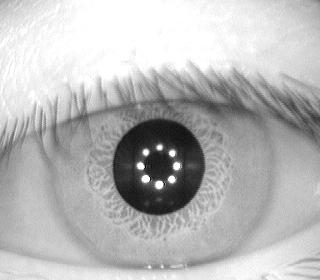
\includegraphics[width=80mm]{Resources/eye-original.jpg}
  \caption{Example of provided image.}
  \label{ImgOriginal}
\end{figure}

\newpage

\subsection{Brightness adjustment}
Images from one camera may exhibit varying brightness levels. 
To standardize the images I change their brightness.
I calculate image brightness as a mean of all pixel values. Then I adjust the brightness to value 50\%.
This normalization process ensures consistent brightness levels for all images, Fig \ref{ImgAdj}.

\begin{figure}[ht!]
  \centering
  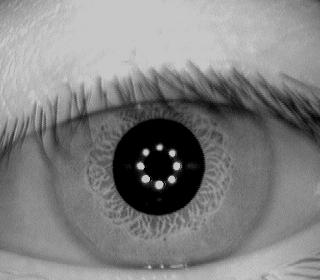
\includegraphics[width=80mm]{Resources/eye-ImgAdj.jpg}
  \caption{Image with changed Brightness}
  \label{ImgAdj}
\end{figure}


\subsection{Smoothing}
High-frequency objects in the image (for ex. eyelashes) can make a lot of noise and edges will be poorly detected.
So to achieve better performances, it's good to smooth image. I use \(12 \times 12 \) Gaussian filter with standard deviation \(\sigma = 15\).
The result of the filter is seen in Fig. \ref{ImgSmooth}.

\begin{figure}[ht!]
  \centering
  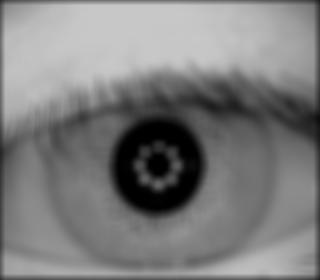
\includegraphics[width=80mm]{Resources/eye-ImgSmooth.jpg}
  \caption{Smoothed image.}
  \label{ImgSmooth}
\end{figure}

\subsection{Edge detection}
To detect edges in the image I use a Canny edge detector with \(threshold = 0.1\).
The edge detector returns a binarized image with edges, Fig. \ref{ImgEdge}.

\begin{figure}[ht!]
  \centering
  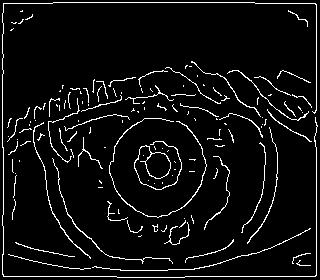
\includegraphics[width=80mm]{Resources/eye-ImgEdge.jpg}
  \caption{Edges of smoothed image.}
  \label{ImgEdge}
\end{figure}

\subsection{Circle Hough Transform}
Circle Hough Transform (CHT) method is based on iterating through the binarized image (where \textit{x} and \textit{y} are coordinates of a non-zero pixel)
and changing parametric space by adding score \(1 \over r \) to the all points that lie in the border of the circle with radius \textit{r} and center \textit{x},\textit{y}.
If the radius is unknown, it should change from \textit{min\_radius} to \textit{max\_radius}.
Example of parametric space, Fig. \ref{abspace}.

\begin{figure}[ht!]
  \centering
  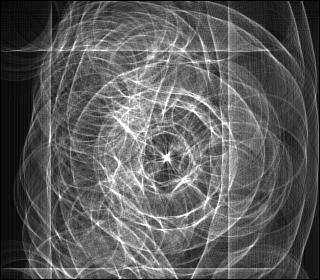
\includegraphics[width=80mm]{Resources/eye-abspace.jpg}
  \caption{Example of parametric space slice with the best circle match.}
  \label{abspace}
\end{figure}

\newpage

\textbf{My hyperparameters of CHT}
\begin{itemize}
  \item \( min\_radius = 25 \)
  \item \( max\_radius = \floor*{\min{(max\_x, max\_y)} \over {2} } \)
  \item \(coordinates\_step = 1 \)
  \item \( radius\_step = 1 \)
\end{itemize}

My implementation is not optimized, it needs ~1.5 min to create an iris template.


\subsection{Circles selection}
The first circle is the circle with the highest rate in parametric space.
The second circle is selected same way (2nd highest rate), but I made several rules to enhance the quality of detection:
\begin{itemize}
  \item Difference between two circles should be more than \textit{circles\_radius\_diff}. It helps skip circles that are almost identical to the 1st circle. I use value \(circles\_radius\_diff = 40\).
  \item The centers of the circles can be spaced a maximum of \textit{circles\_center\_diff} pixels apart on each side. This rule helps discard circles, that are made from noise. In my implementation I use \(circles\_center\_diff = 10\)
  \item Circles shouldn't cross, so I use function \textit{circcirc} to detect crossing points of two circles. If coordinates of crossing are \textit{NaN} then circles don't cross.
\end{itemize}

\noindent Resluts of the segmentation you ca see at figures \ref{ImgSegmented}, \ref{AllSegmented}.

\begin{figure}[ht!]
  \centering
  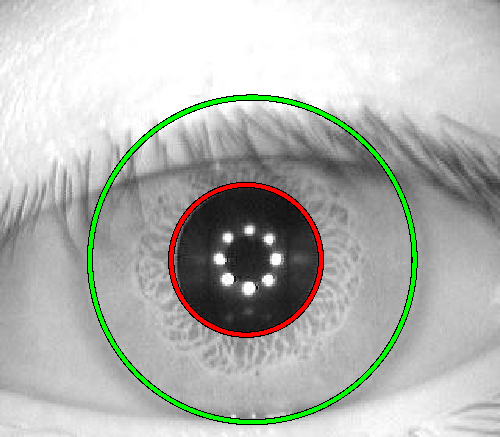
\includegraphics[width=80mm]{Resources/eye-Segmented.png}
  \caption{Segmented iris.}
  \label{ImgSegmented}
\end{figure}

\newpage

\begin{figure}[ht!]
  % \centering
  \includegraphics[width=180mm]{Resources/all-segmented.png}
  \caption{Provided images with iris segmentation.}
  \label{AllSegmented}
\end{figure}




\subsection{Noise removing}
Using the Hough Transform method is possible to detect noise in the segmentated iris, Fig. \ref{ImgNoise}.

\begin{figure}[ht!]
  \centering
  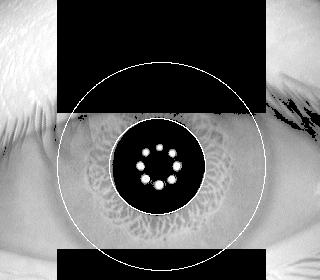
\includegraphics[width=80mm]{Resources/eye-noise.jpg}
  \caption{Removing noise from iris}
  \label{ImgNoise}
\end{figure}

\newpage

\section{Encoding}
The next step is the normalization of the iris image (Fig. \ref{IrisNormal}), transforming into the polar coordinates (Fig. \ref{IrisPolar} ) and creating a template 
using Gabor wavelet phase quantization (Fig. \ref{IrisCode}). 

\begin{figure}[ht!]
  \centering
  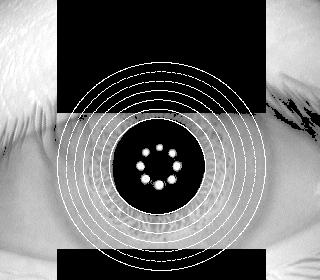
\includegraphics[width=80mm]{Resources/iris-normal.jpg}
  \caption{Iris normalization}
  \label{IrisNormal}
\end{figure}

\begin{figure}[ht!]
  \centering
  \def\svgscale{0.7}
  \includesvg{Resources/iris_polar.svg}
  \caption{Visualization of the iris in polar coordinates.}
  \label{IrisPolar}
\end{figure}

\begin{figure}[ht!]
  \centering
  \def\svgscale{0.7}
  \includesvg{Resources/iris_code.svg}
  \caption{Iris code with noise mask.}
  \label{IrisCode}
\end{figure}

\newpage

\section{Comparison}

\subsection{Hamming distance}
Normalized Hamming Distance (HD) is used for iris comparison.
\begin{equation}
  HD = \lVert (codeA \oplus codeB) \cap maskA \cap maskB \rvert \over \lvert maskA \cap maskB \rvert
\end{equation}

\subsection{Rotation}
The eye can be rotated, so the iris code of the same eye can be different.
For iris rotation, the \textit{circshift} function was used.
Because of phase quantization, makes sense to shift by the even numbers.
In my Implementation I shift iris code by $\pm$ 12 bits with \(shift\_step = 2\)

\newpage

\subsection{Identification of provided iris images in the database}

\begin{table}[h]
  \centering
  \begin{tabular}{ |p{1.1cm}|p{1.6cm}|p{1.3cm}|p{0.8cm}|  }
    \hline
    Image   & Person ID & Eye side & HD    \\
    \hline                            
    x2.jpg  & 1         & L        & 0.100 \\ 
    x1.jpg  & 30        & L        & 0.236 \\ 
    x3.jpg  & 22        & L        & 0.318 \\ 
    x4.jpg  & 13        & L        & 0.000 \\ 
    x5.jpg  & 1         & L        & 0.000 \\ 
    x6.jpg  & 4         & R        & 0.000 \\ 
    x7.jpg  & 27        & L        & 0.222 \\ 
    x8.jpg  & 16        & L        & 0.273 \\ 
    x9.jpg  & 13        & L        & 0.000 \\ 
    x10.jpg & 1         & L        & 0.000 \\ 
    x11.jpg & 1         & L        & 0.000 \\ 
    x12.jpg & 2         & L        & 0.000 \\ 
    x13.jpg & 29        & R        & 0.167 \\ 
    x14.jpg & 1         & L        & 0.000 \\ 
    x15.jpg & 1         & L        & 0.363 \\ 
    x16.jpg & 13        & L        & 0.000 \\ 
    x17.jpg & 4         & R        & 0.335 \\ 
    x18.jpg & 14        & L        & 0.198 \\ 
    x19.jpg & 9         & R        & 0.223 \\ 
    x20.jpg & 10        & R        & 0.195 \\ 
    x21.jpg & 13        & L        & 0.176 \\ 
    x22.jpg & 4         & R        & 0.359 \\ 
    x23.jpg & 4         & R        & 0.332 \\ 
    x24.jpg & 1         & L        & 0.000 \\ 
    x25.jpg & 29        & R        & 0.100 \\ 
    x26.jpg & 28        & R        & 0.143 \\ 
    x27.jpg & 4         & R        & 0.000 \\ 
    x28.jpg & 13        & L        & 0.279 \\ 
    x29.jpg & 28        & R        & 0.216 \\ 
    x30.jpg & 1         & L        & 0.000 \\ 
    x31.jpg & 2         & R        & 0.000 \\ 
    x32.jpg & 1         & L        & 0.000 \\ 
    x33.jpg & 7         & L        & 0.000 \\ 
    \hline              
  \end{tabular}  
  \caption{Identification of the provided images.}      
  \label{provided_images_identification} 
\end{table}



\subsection{All-against-all comparison}
I made 77562 comparisons. I didn't compare the codes that were made from the same image.
\subsubsection{Distributions information}
After all-against-all comparison it is possible to plot distributions on histogram, Fig. \ref{database_distributions}.
The parameters of these distributions you can see in table \ref{distributions_parameters}.

\begin{figure}[htbp] 
  \centering
  \def\svgscale{0.7}
  \includesvg{Resources/database_distributions.svg}
  \caption{Distribution of Hamming Distances.}
  \label{database_distributions}
\end{figure}

\newpage



\begin{table}[h]
  \centering
  \begin{tabular}{ |p{2.3cm}|p{2cm}|p{3cm}|  }
    \hline
    Distribution   & Mean   & Standard deviation \\
    \hline
    Same eye       & 0.2575 & 0.1028             \\
    Different eyes & 0.4719 & 0.0136             \\
    \hline
  \end{tabular}   
  \caption{Parameter of the Normal distributions}  
  \label{distributions_parameters}
\end{table}

\subsubsection{Threshold selcection}
I aim to create an acceptance system with the highest possible level of security.
My focus is on minimizing the False Acceptance Rate (FAR) while maintaining a True Acceptance Rate (TAR) of over 95\%.

\begin{itemize}
  \item Threshold = 0.397956
  \item TPR = 96.34\%
  \item FPR = 0\%
  \item TNR = 100\%
  \item FNR = 3.66\%
\end{itemize}


\begin{figure}[htbp] 
  \centering
  \def\svgscale{0.7}
  \includesvg{Resources/ROC.svg}
  \caption{ROC curve of the logistic regression.}
  \label{ROC}
\end{figure}

\newpage

\begin{figure}[htbp] 
  \centering
  \def\svgscale{0.7}
  \includesvg{Resources/database_distributions-threshold.svg}
  \caption{Distribution of Hamming Distances with the threshold.}
  \label{distributions_threshold}
\end{figure}

\section{System with my iris}
\subsection{Caption}
I captured the iris of both my eyes on the VISTA FA2 camera, Fig. \ref{my_iris_captured_photos}

\begin{figure}[ht!]
  \centering
  \includegraphics[width=80mm]{Resources/MY_IRIS/captured_photos.png}
  \caption{Images of my iris.}
  \label{my_iris_captured_photos}
\end{figure}

\newpage

\subsection{Manual eyes detction}

After that I cropped these images (manual eye detection), Fig \ref{my_iris_captured_photos_cropped}.
During the cropping I understood, that all cropped images should be similar, even if the eye was zoomed more than others, the system can't determine its iris bounds.

\begin{figure}[ht!]
  \centering
  \includegraphics[width=80mm]{Resources/MY_IRIS/captured_photos_cropped.png}
  \caption{Cropped images of my iris.}
  \label{my_iris_captured_photos_cropped}
\end{figure}

\subsection{Segmentation}
After tuning parameters a little bit, I have a segmentation algorithm that works with images taken on the VISTA FA2 camera (Fig. \ref{my_iris_segmentation_process}).

\begin{figure}[ht!]
  \centering
  \def\svgscale{0.7}
  \includesvg {Resources/MY_IRIS/segmentation_process.svg}
  \caption{Segmentation process on my iris.}
  \label{my_iris_segmentation_process}
\end{figure}

\newpage

\textbf{Changed hyperparameters:}
\begin{itemize}
  \item \(irisConfig.loNoiseThreshold = 0.2\)
  \item \(gauss\_kern\_size = 15\)
  \item \(thres = 0.05\)
  \item \(min\_radius = 60\)
  \item \(circles\_center\_diff = 20\)
\end{itemize}

\noindent All images was segmented perfectly, Fig. \ref{my_iris_all_segmented}.


\begin{figure}[ht!]
  \centering
  \includegraphics[width=150mm]{Resources/MY_IRIS/all-segmented.png}
  \caption{Segmentation of all images.}
  \label{my_iris_all_segmented}
\end{figure}

\subsection{Comparison}
I have created a database containing my iris codes.
Then I compared codes from database all-against-all.
The results are plotted on the Fig. \ref{my_iris_distributions}.

\begin{figure}[ht!]
  \centering
  \def\svgscale{0.7}
  \includesvg {Resources/MY_IRIS/my_iris_distributions.svg}
  \caption{Distribution of my iris comparison.}
  \label{my_iris_distributions}
\end{figure}

\newpage

The mean Hamming distance of the left and right eyes is 0.3907.

\begin{itemize}
  \item TPR = 100\%
  \item FPR = 38.89\%
  \item TNR = 61.11\%
  \item FNR = 0\%
\end{itemize}

The high FPR could be because each camera has different quality levels. 
To tackle this, we may need to adjust the threshold for each camera individually to better match their varying qualities.

\bibliographystyle{plain}
\bibliography{references.bib}
\nocite{circle_hough_transform}

\end{document}